% !TEX root = SystemTemplate.tex

\chapter{Overview and concept of operations}

This report covers the project overview, user stories, backlog, design and implementation, development environment, deployment, and documentation for the testing project. 


\section{Scope}
This section gives a brief overview of the system.


\section{Purpose}
The purpose of this program is to run many students' {\tt .cpp} files with given test files, and grade them. 


\subsection{Traversing Subdirectories}
Traversing subdirectories is one of the main components of this system. The program runs a {\tt .cpp} file using test files, and the test files are stored in the current and all the subdirectories containing the "test" keyword.

\subsection{Running the Program Using Test Cases}
The software was designed in the Linux environment provided to the group by the university. 

\subsection{Test Case Generation}
A major update in sprint 2 is test case generation. This allows the user to actually generate psuedo-random test cases.

\subsection{Character String Test Generation}
A large edition to test generation is the creation of tests for a single string of lower case characters up to or exactly a length specified by the user.

\subsection{Run away program testing}
A major edition of imparting a time limit for the test programs to run, and if they exceed this time limit on a test, they will fail that test.

\newpage
\subsection{Handling Presentation Errors}
The program will now examine the test results of each out put program. It will mark a test passed if a few small mistakes in presentation are present:
\begin{enumerate}
\item extra spaces
\item misspelled words (i.e. all letters, not right order; first and last letters are correct)
\item decimal - not enough places is marked as incorrect, but too many is marked as correct if it rounds to the correct value.
\end{enumerate}

\subsection{Menu - driven Testing}
The program will now generate test cases for programs that run off a menu. The specifications for
how the menu is set up in the program are stored in \"filename\".spec

\subsection{Code Coverage}
The program will keep track of how many lines of the tested code were covered by the tests it ran.

\subsection{Code Performance}
The program will also keep track of which functions in the tested program use 10\% or more of the time.

\section{Systems Goals}
The goal of this system is to grade students' {\tt .cpp} file(s) just by typing {\tt grade <filename>.cpp}. The product is built to test the {\tt .cpp} file(s) with all the given {\tt .tst} test files in the current directory and all the subdirectories, and compare the results to the corresponding {\tt .ans} files.

\section{System Overview and Diagram}
Here is a flow diagram showing the implementation process:

\begin{figure}[tbh]
\begin{center}
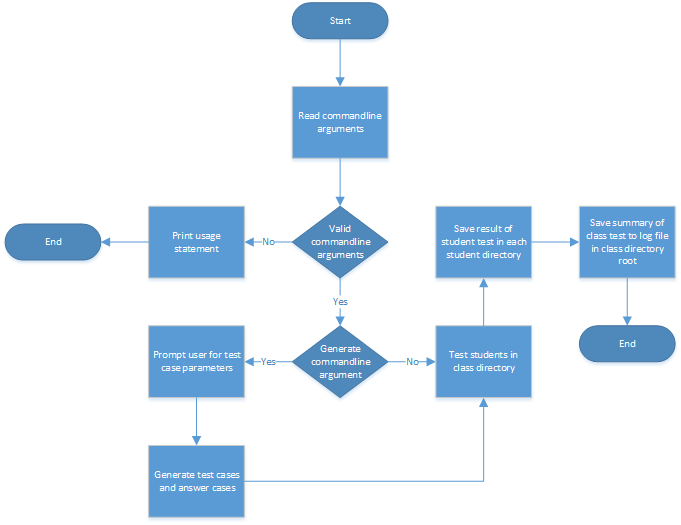
\includegraphics[width=1\textwidth]{./SystemDiagram}
\end{center}
\caption{System Diagram \label{systemdiagram}}
\end{figure}

\section{Technologies Overview}
\begin{itemize}
\item Notepad - Andrew's preferred coding method
\item Notepad++ - Erik's Preferred coding method
\item Netbeans - Jonathan's preferred coding ide
\item gcc - The school's preferred code compiler for c and c++ programs.
\item trello - used to help manage sprint tasks \url{https://trello.com}
\item github - used as a code repository and management system. \url{https://github.com}
\item LaTex - Used to create documentation
\end{itemize}

